\label{fs-eo-impl}


%   The formal model developed ablve can be used for analysis of several systems. 
%  In the previous section, we introduced the formal model that allows describing delivery guarantees in a regular way and proposed necessary and sufficient conditions of~\eo. In this section, we demonstrate how implementations of~\eo\ in state-of-the-art distributed stream processing systems satisfy the necessary condition of~\eo. 

\subsection{MillWheel}

 The $\Gamma$ is all possible streaming {\em records}. Dependency relation $D$ is defined using a graph of user-defined transformations. 
 To ensure fault tolerance,   MillWheel employs a {\em strong productions}~\cite{Akidau:2013:MFS:2536222.2536229}   mechanism that storews persistently  input and output of any operation for each new  input item.
 Thus  each streaming element is saved  before it  may influence other elements or operation states. 
 Recovery function $F$ resends all saved records in case of failure, and each operation deduplicates input  that have been already processed.

The necessary condition of~\eo\ from Theorem~\ref{necessary_conditions} claims that each element $s \in \Gamma$ obtained through a non-commutative operation must be persistently saved before any other element $b_{\tau} \in Cl_D(s)$ that depends on $s$ is released. Strong productions mechanism ensures that this condition is satisfied, i.e. if some element $b_\tau$ is released, it is guaranteed that its dependencies were released earlier (saved to persistent storage). The idea of this method is shown in Figure~\ref{millwheel}. It demonstrates that in MillWheel all elements become recoverable, so there is no need to reprocess them again from an input item in case of failure. 

\begin{figure}[htbp]
  \centering
  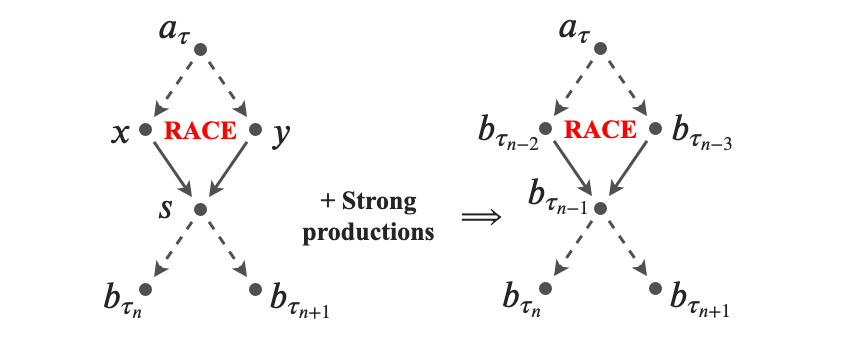
\includegraphics[width=0.48\textwidth]{pics/millwheel}
  \caption{Strong productions mechanism}
  \label{millwheel}
\end{figure}

Such behavior is also called {\em effective determinism}~\cite{akidau2018streaming}, because computations become deterministic until the persistent storage is cleared. Strong productions method guarantees that even if multiple possible results of a non-commutative operation may be obtained due to races, only one of them is actually computed and saved. The price for such~\eo\ enforcement is an overhead on external writes on each transformation in a physical graph.

% This technique allows a developer to use non-deterministic transformations within data flow because the result of this transformation will not be recomputed. This fact relieves from unexpected behavior if a developer does not realize that the code they wrote is non-deterministic.

\subsection{Spark streaming}

In Spark, the  $\Gamma$ is a set of all possible {\em RDD} records. Unlike pure streaming engines like Flink and MillWheel, where input elements arrive one by one, RDD is a small collection of data that is atomically processed. Dependency relation on the power set of $\Gamma$ is also defined using a directed acyclic graph of user operations. Spark inherits main properties form batch processing systems including the fact that each new stage of computations is started only after the previous one is completed. Recovery function $F$ starts reprocessing of a micro-batch from the beginning in case of failure.

The necessary condition for~\eo\ from Theorem~\ref{necessary_conditions} is satisfied because all elements within the micro-batch are released atomically. Elements from various micro-batches can interact only through persistently stored state. Output elements which are ready to be delivered to end-user must wait until the whole micro-batch is completely processed. Therefore, if two output elements $b_{\tau_1},b_{\tau_2} \in Cl_D(s)$ depend on a single item $s$, it is guaranteed that $\tau_1=\tau_2$. The illustration of this behavior is shown in Figure~\ref{spark_flink}. 

% Such behavior significantly increases the processing latency of individual elements~\cite{karimov2018benchmarking}.
 
\begin{figure}[htbp]
  \centering
  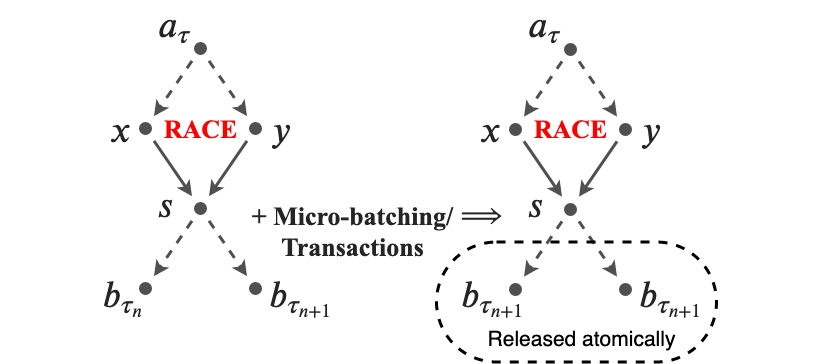
\includegraphics[width=0.48\textwidth]{pics/spark-flink}
  \caption{Micro-batching and transactional approach}
  \label{spark_flink}
\end{figure}
 
\begin{figure*}[tbp]
  \centering
  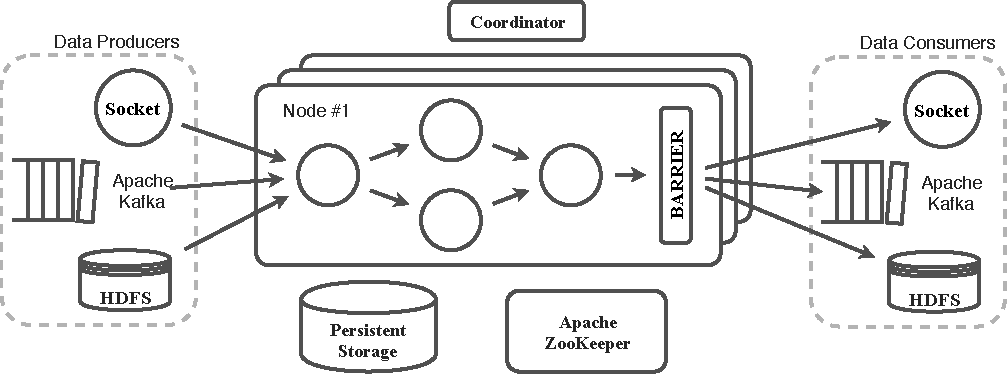
\includegraphics[width=0.78\textwidth]{pics/arch.pdf}
  \caption{The overview of an architecture for drifting state implementation}
  \label {arch}
\end{figure*}
 
% Micro-batching technique ensures determinism as well. To the best of our knowledge, spark streaming is the only state-of-the-art stream processing system that provides for deterministic results. Another advantage of micro-batching is a high throughput~\cite{karimov2018benchmarking}. However, an architecture based on the processing of collections of buffered input elements makes it hard to achieve latency lower than several seconds~\cite{7530084, 7474816}. 

\subsection{Flink}

In Flink, the  $\Gamma$ is represented as all {\em StreamRecords}. Relation $D$ is defined in the form of a directed acyclic graph consisted of user operations. Flink periodically saves information needed for recovery by injecting special elements called {\em checkpoints} into the input stream. Periods between checkpoint are called {\em epochs}. Checkpoints go through the same network channels as ordinary elements and push all inverted dependencies of inputs through the system. Each operation prepares data to save independently at the moment of checkpoint arrival. Prepared data is committed to external storage when checkpoint passes through the whole data flow. Output elements are delivered to end-user only after the commit. Recovery function $F$ reprocesses last non-complete epochs.

This mechanism ensures that all elements within an epoch are processed atomically and all interaction between elements from different epochs are possible only through persistent state. Hence, as it is shown in Figure~\ref{spark_flink}, if two output elements $b_{\tau_1},b_{\tau_2} \in Cl_D(s)$ depend on a single item $s$, it is guaranteed that $\tau_1=\tau_2$. This fact ensures that the necessary condition of~\eo\ from Theorem~\ref{necessary_conditions} is satisfied. Such method is quite similar to the micro-batching technique used in Spark, but in this case, elements are buffered after their processing is done. Another distinction is that multiple epochs can be processed simultaneously. These facts allow Flink to achieve lower latency in comparison with micro-batching, because at the end of an epoch, most of the elements which belong to this epoch, has already been processed.

% A strong advantage of such technique is that it does not degrade throughput. This method also allows a developer to use non-deterministic transformations in data flow because results can be observed only after commit. However, as in the micro-batching approach, ready-to-release output elements must wait until the epoch is committed.  Besides, checkpoints cause extra latency overhead because an operation with multiple inputs must wait until checkpoints arrive from each input. Only after that, an operation can safely send checkpoint further. This behavior is known as {\em checkpoints alignment}~\cite{Carbone:2017:SMA:3137765.3137777}.